\documentclass[twocolumn]{article}

\usepackage{graphicx}

\begin{document}
%title
\title{Dead Reckoning with Adaptive (Fuzzy) Calibration}
\author{ Devin Smittle \\ University of Missouri \\
  dzs6w3@mail.missouri.edu \and Veselin Georgiev \\ Southeast Missouri
  State University \\ vvgeorgiev2s@semo.edu} \date{\today}
\maketitle

%abstract
\begin{abstract}
  \emph{This paper discusses using an accelerometer in smart-phones to
    determine position where GPS falters. The idea is to train an
    artificial intelligence so that it can determine a phone's
    movement solely given an accelerometer. We eliminate the use of a
    compass since a person can hold a phone in any manner whilst
    moving. In a general situation, for our purpose, a compass is
    utterly unreliable.}
\end{abstract}

\section{Introduction}

This is the introduction.

\begin{center}

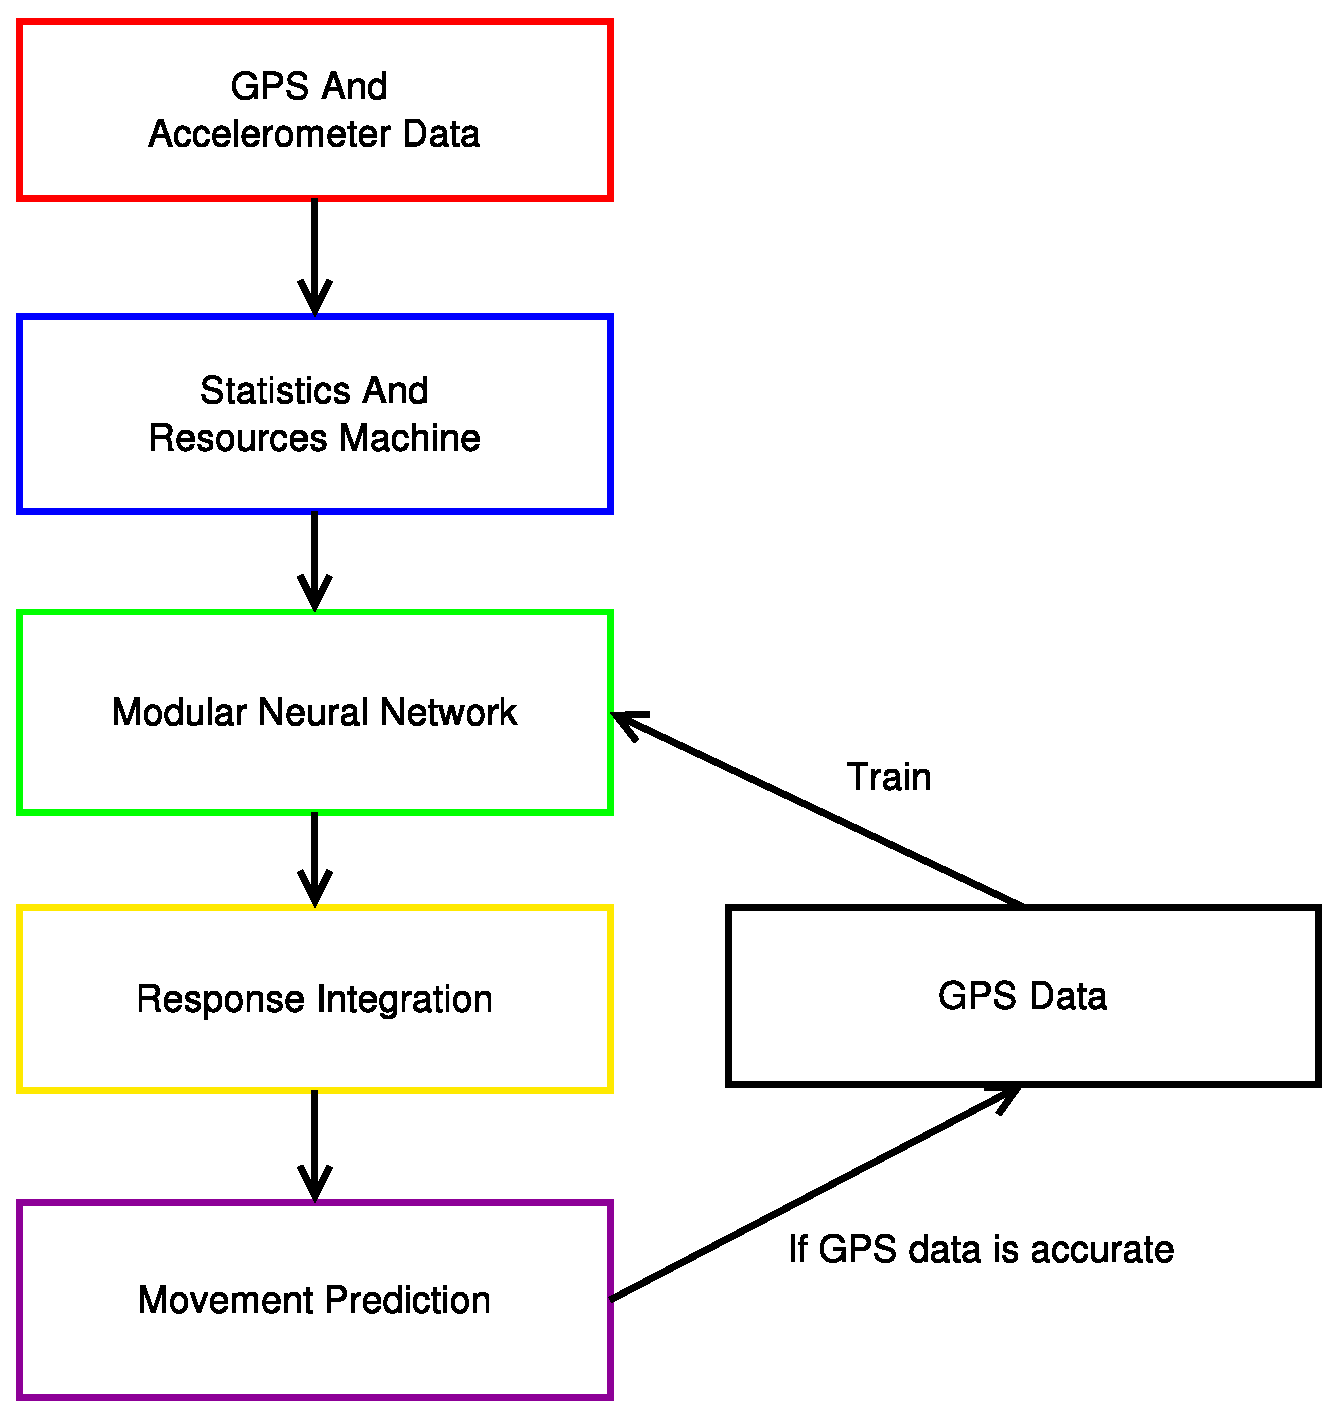
\includegraphics[width=0.9\columnwidth,keepaspectratio]{../figures/process_diagram/process}
\\
Figure 1.
  
\end{center}


\section{Data}
hmm..

% bibliography
\begin{thebibliography}{9}
\bibitem{duke}
  Ionut Constandache \and Romit Roy Choudhury \and Injong Rhee
  \emph{Toward Mobile Phone Localization without War-Driving}
\bibitem{melin}
  Patricia Melin \and Oscar Castillo
  \emph{Hybrid Intelligent Systems for Pattern Recognition}
\end{thebibliography}

\end{document}